\section{Design and Implementation }

\subsection{Hardware ans Software}
This was run on a MacBook Pro computer using Iverilog. Additionally, gtkwave was used to monitor the modules input and outputs.

\subsection{TSC design overview}

The TSC (Trigger Surround Cache) has a 3 bit state register, a 32-bit timer,
a 32-bit TRIGGER\_TM, and an internal ring buffer.
It is connected to the ADC (Analog-to-Digital Converter)
via a request (REQ), ready (RDY), and data (DAT) lines.
Additionally, the TSC can communicate with other devices using triggered (TRD), Send Buffer (SBF),
serial data (SD), and completed data (CD) registers and wires.


\begin{figure}[H]
      \centering
      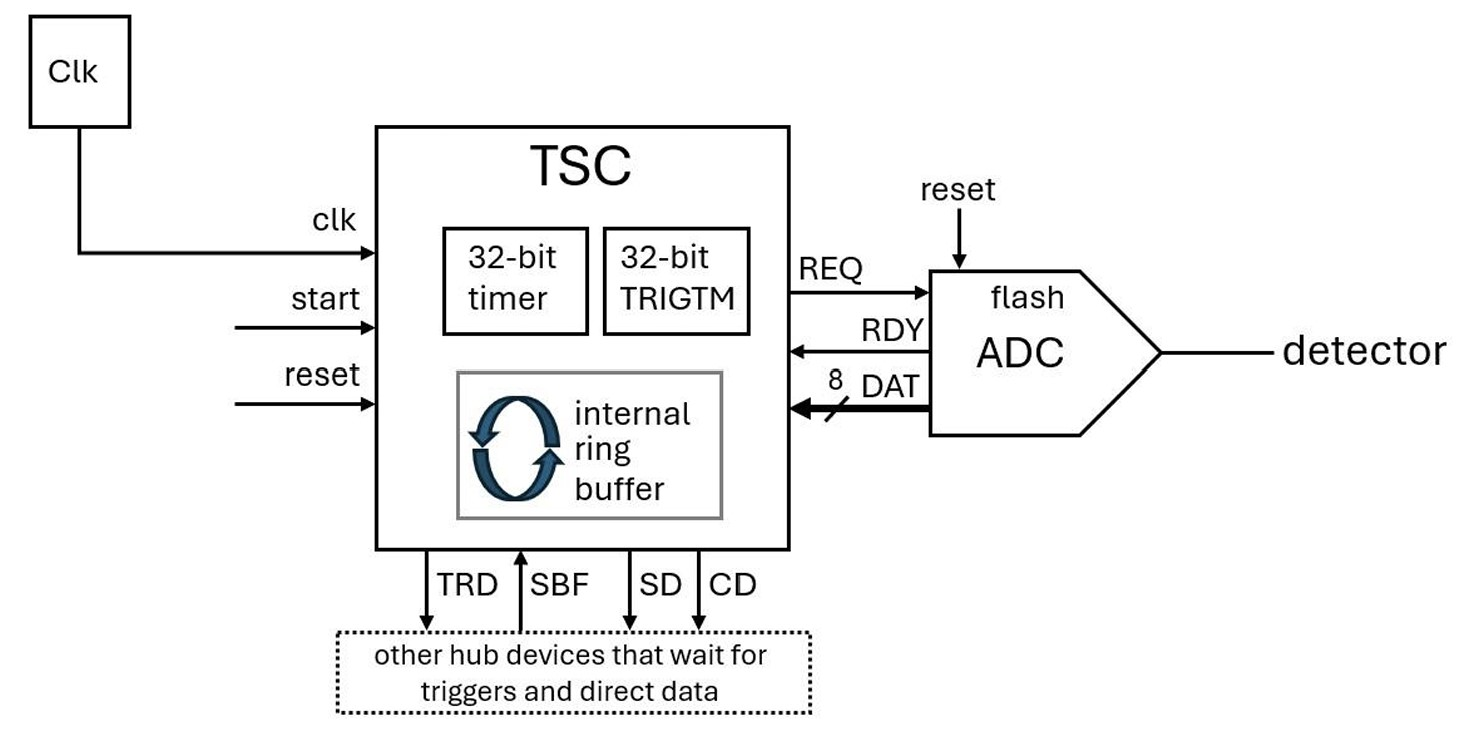
\includegraphics[width=0.8\columnwidth]{Figures/block_diagram_of_TSC}
      \caption{Block diagram of the TSC}
      \label{fig:block diagram of TSC}
\end{figure}

There is also an accompanying TSC\_tb test bench which is used to initiate and test the TSC module.

\subsection{CLock (clk)}
A 250 MHz clock signal is set up on clk wire in the TS\_tb test bench.

\subsubsection{State register}
The state register is a 3-bit register that has the folowing states:
\begin{itemize}
      \item STOP (0b000) :
            State when the machine is powered on and has not been reset yet.
      \item READY (0b001) :
            State that is enter on the reset pin rising edge and it waits for the start pin rising edge.
      \item RUNNING (0b010):
            State that is entered from ready or Idle state once the start pin rising edge is pulled hight.
            It incrementing the timer and wright adc values to the ring buffer.
      \item TRIGGERED (0b011):
            State entered when the value read from the ADC is
            greater than the predetermined trigger value (TRIGVL).
            It capturing the next 16 values.
      \item IDLE (0b100);
            This state is entered when a trigger event has occurred
            and the TSC is waiting for the start pin or SPF pins rising edge.
      \item SENDING (0b101):
            This state is entered from the IDLE state when the SFB line it pulled high.
            It indicates that data is being sent on the SD line.
\end{itemize}


\subsubsection{Timer}
The timer is incremented on the rising edge of the clock. When
a trigger even occurs the timer is save in the TRIGTM register which is outputted to the test bench.
The timer is reset if a transition into a running state occurs.
To calculate the time store in the TRIGTM register the timer is multiplied by the clock period (4 ps).


\subsubsection{Ring Buffer}
The ring buffer is used to store the values read by the ADC.
It is made up of 32 8-bit registers stored in an array called ring\_buffer.
The tail pointer is named write\_prt and is Initial set to 5'b11111.
and the head pointer is named read\_ptr and is initial set to 5'b00000.
The 5 bit format for the head and tail index is used to induce role offer at value 32 (32 just becomes 0).
To add a new value to the ring buffer the write\_ptr is incremented and then the
value is stored in the ring buffer at the write\_ptr index then read\_ptr is incremented.
To read a value from the ring buffer the value at the read\_ptr index is read and the read\_ptr is incremented.
this proses is repeated until the read\_prt = wright\_ptr. Indicates that all the values have been read.

\subsubsection{How the TSC intervacec with the ADC}
The ADC is initialized in the TSC module.
This connect the adc\_request to REQ, adc\_request to RST,  adc\_ready to RDY, and adc\_data to DAT.
The adc\_request line is connected to the main reset line this mean that the ADC module is reset when the TSC\_td
module is pull the reset line hight.
once the ADC is reset the ADC will pull the adc\_ready line hight to indicate that the ADC is ready to send data over the 8 bit DAT line.
The  bytes of of data being sent over the DAT line are extracted from a CSV file in the ADC module.
When the TSC module detects the adc\_ready line is hight and the TSC is in the running state.
The TSC will pull the adc\_request line hight on the posedge of the clk line for 1 ps to request data from the ADC on the adc\_data line.
This can be seen in the two code section named \ref{posedgeadcready} and \ref{clockrunning} below.
The subsequent data is then stored on the ring buffer.


\begin{lstlisting}[language=Verilog, caption={Code for storing data and moving pointers in the posedge adc\_ready}, label={posedgeadcready}]
      always @(posedge adc_ready) begin
            if (adc_request) begin
            #1 //delay so the pulse doesn't disappear on the echo. TO BE REMOVED
          
            //manage trigger_value
            //... the trigger code is here

      //store data and move pointers around
      ring_buffer[++write_ptr] = adc_data;
      read_ptr++;

      adc_request = 0; //pull request down
    end
  end
\end{lstlisting}


\begin{lstlisting}[language=Verilog, caption={Code for requesting data from the ADC on posedge of the clock when in RUNNING state}, label={clockrunning}]
      `RUNNING: begin
        timer++;
        if (~ adc_request)
          adc_request = 1; //request new adc value (handled with posedge adc_ready)
      end
\end{lstlisting}




\subsubsection{Triggering}

The TSC module has a trigger value (TRIGVL) that is set in TSB module.
However, TRIGVL can also be set in the TSC\_tb.
When the TSC is in the RUNNING state and the ADC is outputing to adc\_data if the value adc\_data is
greater than the TRIGVL the following event will occurs:

\begin{itemize}
      \item The TSC module transitions to the TRIGGERED state.
      \item The TRIGTM register is set to the current value of the timer.
      \item  The reg remaining\_values is set to equal 5'h10 (16 in decimal). This is done to help record 16 more values.
\end{itemize}

This Implementation is demonstrated in the code below.

\begin{lstlisting}[language=Verilog, caption={Code for triggering event in the TSC module}, label={triggering}]
      if (state != `TRIGERED) begin  //if it hasn't been triggered already, check for a valid trigger
        if (adc_data > TRIGVL) begin
          state = `TRIGERED;
          TRIGTM = timer; //capture time of trigger
          remaining_values = 5'h10; //set remaining adc values to 16 (handled by posedge clk)
        end
      end
\end{lstlisting}


When the TSC module is in the TRIGGERED state the TSC dose the following on the positive edge fo the clock.
It incremented the timer value because as per project brief the timer must only stop being incremented once the IDLE stat has been entered.
Then the TSC will check if remaining\_values =0 to see if 16 byte have been recorded.
If all 16 bytes have been recoded it will transition to the IDLE state.
else it will pull the adc\_request line hight to request more data from the ADC and decrease the remaining\_values by 1 to
indicate that it has recorded one more value. This this can be seen in the code below.

\begin{lstlisting}[language=Verilog, caption={Code for triggering event in the TSC module}, label={triggering}]
      `TRIGERED: begin
        timer++;
        if(remaining_values--) begin //check that there are remaining values left to capture and decrement.
          if (~ adc_request)
            adc_request = 1; //request new adc value (handled with posedge adc_ready)
        end else begin //all 16 values have been captured, wait for start or SBF command
          state = `IDLE; 
          TRD = 1'b1;
        end
      end
\end{lstlisting}

\subsubsection{Sending data to to HUB devices}
If the TSC module is in the IDLE state and the SBF line is pulled hight the TSC module will transition to the SENDING state.
durint this transition it will set SD hight and CD low
















